\documentclass[12pt]{article}
\usepackage[english]{babel}
\usepackage{color}
\usepackage{amsmath,amssymb,amsfonts,textcomp}
\usepackage{graphicx}
\usepackage{hyperref}
\usepackage{float}
\usepackage{caption}
\usepackage[round]{natbib}
\usepackage{Sweave}
%\usepackage{C:/Users/Erick/Documents/conffallchap/Sweave}
\usepackage{setspace}
%\doublespacing
%Begin commands from Journal of statistical software
\def\@codex#1{{\normalfont\ttfamily\hyphenchar\font=-1 #1}\egroup}
\makeatother
\let\code=\texttt
\let\proglang=\textsf
\newcommand{\pkg}[1]{{\fontseries{b}\selectfont #1}}
%END commands from Journal of statistical software
%%  Sweave specific commands
% make the input blue, output red
\DefineVerbatimEnvironment{Soutput}{Verbatim}{formatcom=\color{blue}}
\DefineVerbatimEnvironment{Sinput}{Verbatim}{fontshape=sl, 
	formatcom=\color{red}}

	
\title{Econometrics of XYZ Using R}
%\author{Author1, Author2, Author3}
\author{ {Author1}\footnote{corresponding author. 
 Professor of Economics at ABC University, 
Director:  Ab Institute, 123 Hillside Ave, New York, NY 11234, USA. Phone: 718-555-4065, fax: 718-555-3518, e-mail: \url{author1@ABC.edu}.} 
\and 
{Author2}\footnote{PhD, CEO, YYY Analytics. 2 Corporate Drive, Suite 254, mytown CT 06484, USA. Phone (203) 555 9157, fax: (203) 555 3643, e-mail: \url{author2@YYYanalytics.com}.}
\thanks{We thank Mrs. Jane Smith for valuable assistance and colleagues for valuable comments.} 
} %end of author list and thanks

%% Please  INCLUDE FULL NAME AFFILIATION AND ADDRESS FOR EACH AUTHOR AND THANKS IF ANY

	
\begin{document}
\Sconcordance{concordance:sample1.tex:sample1.Rnw:%
1 160 1 1 2 13 0 1 2 3 1 1 2 7 0 1 2 13 1 1 2 1 0 3 1 31 0 1 2 189 1}


\maketitle

\begin{abstract}
We develop econometric methods for an  important
econometric issue.
We illustrate its application using an R package `xxyy'
and recent data.
This paper also illustrates the use of R in macro-econometrics.
--sample text -- sample text----
--sample text -- sample text----
THIS IS A LATEX TEMPLATE FOR VOLUME 41 OF HANDBOOK OF STATISTICS


AUTHORS' MAILING ADDRESS DETAILS MAY BE COMMENTED OUT IN THE CHAPTER
 BUT ARE NEEDED BY THE PUBLISHER
 --sample text -- sample text----

\bigskip

Keywords: Private Investment; Time series; Bootstrapping


\end{abstract}

\section{Introduction}
xyz is an important unsolved problem in Econometrics.
The aim of this paper is threefold.
--sample text -- sample text----
--
THIS IS A LATEX TEMPLATE FOR VOLUME 41 OF HANDBOOK OF STATISTICS

AUTHORS' MAILING  ADDRESS DETAILS MAY BE COMMENTED OUT IN THE CHAPTER BUT ARE NEEDED BY THE PUBLISHER

Now, we show how to include a figure in the paper and
how to refer to it.  The folder should have the 
file named `figCVS.pdf' for the following to work.

\begin{figure}[ht!]
\centering 
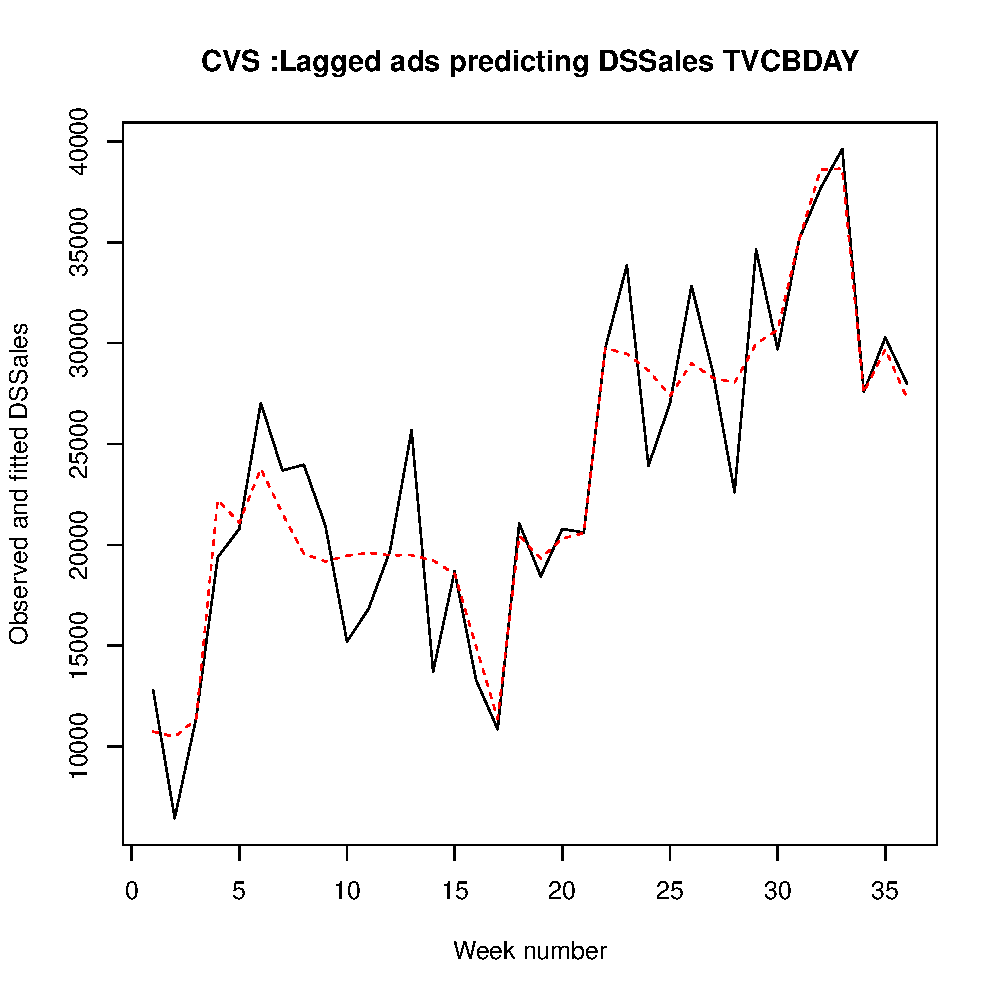
\includegraphics[width=1\textwidth]{figCVS.pdf}
\caption{Excellent fit by kernel regressions}
\label{fig.fit}
\end{figure}
Figure  \ref{fig.fit} shows how the kernel regression fit is
excellent compared to OLS.

\section{Review of Stylized Facts}
See Table \ref{tab.lit} for a review of some stylized facts.

THIS TEMPLATE shows one way of including a table containing text
in a Latex document.


\begin{table}[ht]
\caption{Stylized facts of major interest rates in India} 
\centering
\resizebox{\textwidth}{!}{
\begin{tabular}{ll}
	\hline
Interest rates & Stylized Facts\\
\hline
\hline
 Call money market rate & Usually exhibits large volatility\\ 
 Bank rate & Usually non-varying in nature \\ 
 Prime Lending rate	& A potential indicator of long term rate and exhibits stickiness\\ 
 Redemption yield -& A potential indicator of long term rate in case of shift from -\\
 on Government securities& seigniorage financing to bond financing of fiscal deficit \\
 Treasury Bills rate & A significant reference rate in the short term \\ 
 \hline
 \footnotesize Source: Author's analysis
 \end{tabular}
 }
 \label{tab.lit}
\end{table}

\section{Frish's Problem and Rao's Solution}
--sample file -- sample file----
--sample file -- sample file----

Linear regressions are common in Econometrics even though
nonlinear nonparametric methods are receiving attention these days.
Ragnar Frisch, winner of 1969 Nobel in Economics,
had posed the following problem before the
Oxford Conference of the Econometric Society in September 1936. Let
$x_1$ and $x_2$ be two variables such that
\begin{eqnarray}
\label{eq.frisch}
x_1 &= a \xi + \epsilon_1, \nonumber \\
x_2 &= b \xi + \epsilon_2,
\end{eqnarray}
where $\xi, \epsilon_1, \epsilon_2$ are independent random variables,
and where $a, b$ are unknown constants.  Frish's problem
was: What are the conditions under which the regression of $x_1$ on
$x_2$ is linear?


\cite{Rao47} and \cite{Rao49} 
assume that: (i) expectations $E(\xi), E(\epsilon_1),$ 
and $E(\epsilon_2)$ exist, (ii) $\epsilon_2$ is independent of $\xi$ and $\epsilon_1$,
and (iii) the conditional expectation, $E(\epsilon_1 |\xi)=0$, while $\epsilon_1$ is not necessarily
independent of $\xi$.  Rao then proved that
the necessary and sufficient condition for
the regression of $x_1$ on
$x_2$ to be linear, whatever may be the constants ($a, b$), is that
the characteristic function of  $\xi$ is $exp[c|t|^d]$ 
and the characteristic function of  $\epsilon_2$ is $exp[c^\prime|t|^d]$.

\section{Application to cars data}
--sample file -- sample file----
--sample file -- sample file----
We let $y$ be the stopping distance of a car (in feet),
and $x$ be the speed of the car in miles per hour, using 
Ezekeil's data called `cars' always available in R. 
We are regressing $y$ on $x$ to show that faster a car is driving
longer is the distance before it comes to a full stop.

Our first R input code is:

\begin{Schunk}
\begin{Sinput}
> rbind(head(cars,3),tail(cars,3)) # first \& last 3 row of data
\end{Sinput}
\begin{Soutput}
   speed dist
1      4    2
2      4   10
3      7    4
48    24   93
49    24  120
50    25   85
\end{Soutput}
\end{Schunk}

We have combined the first and last three rows of data for brevity in
the following R output.

\begin{Schunk}
\begin{Sinput}
> nrow(cars)
\end{Sinput}
\begin{Soutput}
[1] 50
\end{Soutput}
\end{Schunk}

The R output above shows that `cars' data in R has $p=1, T=50$.
Instead of reporting the  (50$\times 2$) $X$ matrix,
brevity demands that we report the first three and last three rows of data. 

The simplest linear regression for cars data using R
is implemented by `lm' function creating an R object called `reg'
in the R code below.
\begin{Sinput}
library(stargazer)	
attach(cars) #to access columns by name
reg=lm(dist~speed) #standard R method for regression
stargazer(reg)
\end{Sinput}

The output of the above code is in a form suitable to produce
the following (Latex) Table \ref{tab.reg} where standard errors
of regression coefficients are in parentheses under the coefficient
values.
% Date and time: Tue, May 01, 2018 - 12:20:14 PM
\begin{table}[!htbp] \centering 
\caption{Regression of stopping distance on speed by standard R method} 
\label{tab.reg} 
\begin{tabular}{@{\extracolsep{5pt}}lc} 
	\\[-1.8ex]\hline 
	\hline \\[-1.8ex] 
& \multicolumn{1}{c}{\textit{Dependent variable:}} \\ 
\cline{2-2} 
\\[-1.8ex] & dist \\ 
\hline \\[-1.8ex] 
speed & 3.932$^{***}$ \\ 
& (0.416) \\ 
& \\ 
Constant & $-$17.579$^{**}$ \\ 
& (6.758) \\ 
& \\ 
\hline \\[-1.8ex] 
Observations & 50 \\ 
R$^{2}$ & 0.651 \\ 
Adjusted R$^{2}$ & 0.644 \\ 
Residual Std. Error & 15.380 (df = 48) \\ 
F Statistic & 89.567$^{***}$ (df = 1; 48) \\ 
\hline 
\hline \\[-1.8ex] 
\textit{Note:}  & \multicolumn{1}{r}{$^{*}$p$<$0.1; $^{**}$p$<$0.05; $^{***}$p$<$0.01} \\ 
\end{tabular} 
\end{table} 

\section{Summary and Final Remarks}
This chapter has attempted to solve an important econometric
problem and illustrated its solution using R.


THIS IS A LATEX TEMPLATE FOR VOLUME 41 OF HANDBOOK OF STATISTICS
--sample text -- sample text----

--sample text -- sample text----

\cite{Vinodb93} illustrates how to cite an article in a collection.

\cite{Vinodu07} illustrates how to cite an unpublished article.

\cite{R18} illustrates how to cite a book or an electronic document
in the form of a book.

Please see the Ref-sample.bib file in the folder for the exact format to type
references into a *.bib file.	



\bibliographystyle{elsarticle-harv}
\bibliography{Ref-sample}


\end{document}

%%%%%%
%%%%%%
%%%%%%
%%%%%%
%%%%%%
%%%%%%
%%%%%%
%%%%%%
%%%%%%
%%%%%%
%%%%%%
%%%%%%
%%%%%%
%%%%%%
%%%%%%
%%%%%%
%%%%%%
%%%%%%
%%%%%%
%%%%%%
%%%%%%
%%%%%%
%%%%%%
%%%%%%
%%%%%%
%%%%%%
%%%%%%
%%%%%%
%%%%%%
%%%%%%
%%%%%%
%%%%%%
%%%%%%
%%%%%%
%%%%%%
%%%%%%
%%%%%%
%%%%%%
%%%%%%
%%%%%%
%%%%%%
%%%%%%
%%%%%%
%%%%%%
%%%%%%
%%%%%%
%%%%%%
%%%%%%
%%%%%%
%%%%%%
%%%%%%
%%%%%%
%%%%%% 
%%%%%%
%%%%%%
%%%%%%
%%%%%%

library(generalCorr)
options(np.messages=FALSE)
set.seed(34)
y=sample(1:25)
x1=sample(1:25)
x2=sample(1:25)
x3=sample(1:25)
library(xtable)
out1=causeSummary(cbind(y,x1,x2),ctrl=x3)
xtable(ou1)
  
\begin{figure}[!htpb]
	\begin{center}
		\centering
		\caption{Total Units Sold}\label{fig:AllUnits}
		\includegraphics[width=0.90\textwidth, totalheight=0.3\textheight]{all_units}
		\captionsetup{width=0.90\textwidth, singlelinecheck=off,font=scriptsize}
		\caption*{\scriptsize{Total aggregated cold remedies units sold at CVS, Kmart, Meijer, Rite Aid, Target, Walgreens and WalMart. Weekly data from January 2011 to October 2013.}}
	\end{center}
\end{figure} 
\begin{table}[h]
\centering
\caption{Results when interest rates are CPI based Inflation Adjusted}
\hline
\hline
\begin{(subtable}
	\subfloat{3a. Generalized Correlation Results}{
		\begin{tabular}{c c c c c}
			\hline
			cause & Response & Strength & Correlation & p-value\\
			\hline
			Private Investment & Public Investment & 44.882 & 0.9603 & 0.00\\ 
			Treasury Bills rate & Private Investment & 100.000 & 0.5375 & 0.01453\\
			\hline
		\end{tabular}
		\label{table:GenCorr}
	\end{subtable}
	\begin{(subtable}
		\subfloat{3b. Generalized Correlation Results}{
			\begin{tabular}{c c c c c}
				\hline
				cause & Response & Strength & Correlation & p-value\\
				\hline
				Private Investment & Public Investment & 44.882 & 0.9603 & 0.00\\ 
				Private Investment & Long Term Yield rate & 100.000 & 0.5548 & 0.01111\\
				\hline
			\end{tabular}
			\label{table:GenCorr}
		\end{subtable}
		\begin{(subtable}
			\subfloat{3c. Generalized Correlation Results}{
				\begin{tabular}{c c c c c}
					\hline
					cause & Response & Strength & Correlation & p-value\\
					\hline
					Private Investment & Public Infrastructure & 100.000 & 0.9343 & 0.00\\ 
					&Investment& & &\\
					Treasury Bills rate & Private Investment & 100.000 & 0.5375 & 0.01453\\
					\hline
				\end{tabular}
				\label{table:GenCorr}
			\end{subtable}
			\begin{(subtable}
				\subfloat{3d. Generalized Correlation Results}{
					\begin{tabular}{c c c c c}
						\hline
						cause & Response & Strength & Correlation & p-value\\
						\hline
						Private Investment & Public Infrastructure & 100.000 & 0.9343 & 0.00\\
						&Investment& & &\\
						Private Investment & Long Term Yield rate & 100.000 & 0.5548 & 0.01111\\
						\hline
					\end{tabular}
					\label{table:GenCorr}
				\end{subtable}
				\begin{(subtable}
					\subfloat{3e. Generalized Correlation Results}{
						\begin{tabular}{c c c c c}
							\hline
							cause & Response & Strength & Correlation & p-value\\
							\hline
							Private Investment & Public Non & 100.000 & 0.9533 & 0.00\\ 
							&-Infrastructure Investment& & &\\
							Treasury Bills rate & Private Investment & 100.000 & 0.5375 & 0.01453\\
							\hline
						\end{tabular}
						\label{table:GenCorr}
					\end{subtable}
          \begin{(subtable}
						\subfloat{3f. Generalized Correlation Results}{
							\begin{tabular}{c c c c c}
								\hline
								cause & Response & Strength & Correlation & p-value\\
								\hline
								Private Investment & Public Non & 100.000 & 0.9533 & 0.00\\
								&-Infrastructure Investment& & &\\
								Private Investment & Long Term Yield rate & 100.000 & 0.5548 & 0.01111\\
								\hline
							\end{tabular}
							\label{table:GenCorr}
						\end{subtable}
						\label{table:GenCorr}
					\end{table}
